
\chapter{Introduction}
\label{cha:intro}

This document provides the user with a basic understanding of the
architecture, the features and the operations of \rtd\ and the
associated \ee\ Kernel.

\rtd\ is now fully integrated with the open source Eclipse framework,
as is distributed as a set of plugins that can be installed on top of
various Eclipse versions.

This document covers the description of two main components of \rtd,
which are the code generator plugins for OSEK/VDX systems and the
schedulability analysis plugins.

The Code generator plugins consists of a {\em core} component,
required for all operations, and a number of plugins providing time
verification and automatic generation of the implementation of
real-time embedded software.

The Schedulability analysis plugins provides schedulability analysis
support, allowing the user to model the application architecture using
the \rtd\ metamodel. Once modeled, the system can be analyzed using
the schedulability tests, providing in this way useful information
such as task response times, and sensitivity analysis.


\section{Software design with \rtd{}}

The architecture of \rtd\ is shown in Figure
\ref{fig:rtdruid-plugin-architecture}. Model information (i.e. for
both the functional and the architecture-level components) is stored
in an internal repository and it is made available by means of an open
format based on XML.

The toolset architecture is based on a kernel, or Core module, providing
management of internal data structure and basic services for GUI and
additional plugin modules.

Plugins exploit kernel services in order to provide support to the
design stages in a completely independent way. Here is a list of the
plugins currently available:

\begin{itemize}
\item \rtd\ Modeler;
\item \rtd\ Schedulability Analyzer;
\item \rtd\ Code generator from OIL/AUTOSAR XML;
\end{itemize}
%
\begin{figure}
\begin{center}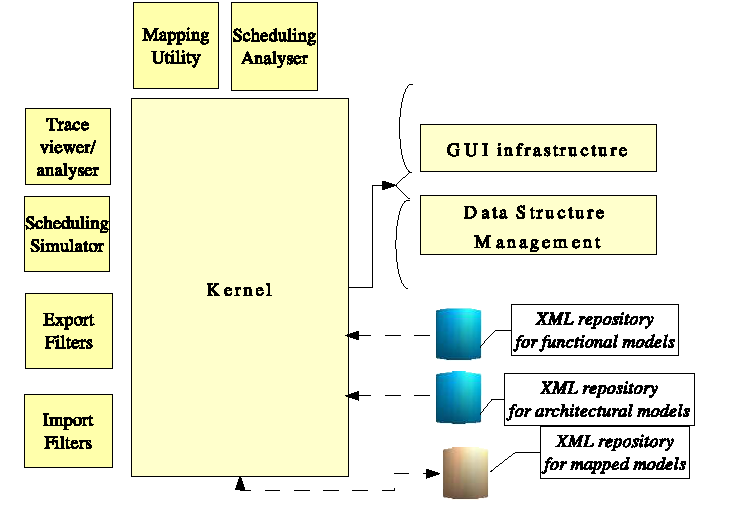
\includegraphics[%
  scale=0.7,bb=0 0 736 529]{images/rtd_plugin_arch.png}\end{center}
\caption{\label{fig:rtdruid-plugin-architecture}The plug-in architecture of \rtd.}
\end{figure}



\section{The open architecture of the \rtd\ tool}

%
\rtd\ allows saving all system information in an open XML
format. Information about the system model, configuration information
and the result of operations performed by plug-in tools, such as
schedulability analysis, tracing or debugging info, can easily be made
available to external or third party tools. Similarly, OIL files can
be imported from or exported to third party products.


\section{\rtd\ integration with Eclipse}

\rtd\ is entirely written in Java. It is based on well-known
development frameworks such as Eclipse, the framework originally
propoted by IBM and now released as an open source development
environment \cite{Eclipse}, and on the W3C XML standard. The \rtd\ tool
makes use of several Eclipse plug-ins, including EMF
\cite{Eclipse-EMF}, GEF \cite{Eclipse-GEF} and CDT
\cite{Eclipse-CDT}\footnote{CDT is the Eclipse component in charge of
C/C++ project management.}.

The integration of \rtd\ with the Eclipse framework easily allows any
user to perform the operations of editing, compiling, debugging and
running the software. The required commands and action sequences are
those common to all Eclipse projects, including CDT.


\section{Content of this document}

The document is divided in two parts. The first one is
dedicated to the code generator plugins, whereas the second one is
dedicated to the schedulability analysis plugins.

The first part about the code generator plugins contains the basic
information for operating with the tool and providing the right
configuration input for the code generation phase. 

In Chapter \ref{cha:overview}, the code generator plugins are
introduced, the code generation process is outlined and the
relationships among the products and the Eclipse development
environment are explained.

Chapter \ref{cha:creating-rtdruid-project} explains the basic steps
that are necessary to start an Rt-Druid project and how to define the
basic configuration info that is required by the tool. A fundamental
part of the configuration tool is contained in the OIL input
file. Syntax and methods for generating the OIL description of the
system are the subject of Chapter \ref{cha:oil-syntax}. The
\ee\ specific extensions to the OIL language that are necessary to
define task placement and other features of multicore systems are
described in Section \ref{sec:oil-multicore}.

The operations that are required for the code generation phase,
together with a detailed description of the input and output data at
each step is the subject of the Chapter \ref{cha:code-generation}.
The kernel configuration and the explanation of the programming model
that needs to be used for \rtd/\ee\ applications are also described in
Chapter \ref{cha:code-generation}.

Finally, the first part of the document concludes with a description
of the \rtd\ standalone version, which is a command-line version of
the code generation plugins, to be used without the Eclipse graphical
interface (see Chapter \ref{cha:Commandline}).

The second part of the document is related to the Schedulability
analysis plugins. The second part starts with Chapter
\ref{cha:schedulability-analysis-introduction}, which gives an
introduction to the purpose of the Schedulability Analysis
plugins. After that, the RT-Druid input file is described in detail
(Chapter \ref{cha:DTD-Input-file}).

Finally, Appendix \ref{cha:Script-File} contains a description of the
ANT scripting support, which enables to run most of the RT-Druid
operations batch. Appendix \ref{cha:oil-definition} contains a
comprehensive OIL implementation description that can be used as a
startup reference.

